%**************************************%
%*    Generated from PreTeXt source   *%
%*    on 2019-04-24T14:42:46-04:00    *%
%*                                    *%
%*   http://mathbook.pugetsound.edu   *%
%*                                    *%
%**************************************%
\documentclass[10pt,]{book}
%% Custom Preamble Entries, early (use latex.preamble.early)
%% Default LaTeX packages
%%   1.  always employed (or nearly so) for some purpose, or
%%   2.  a stylewriter may assume their presence
\usepackage{geometry}
%% Some aspects of the preamble are conditional,
%% the LaTeX engine is one such determinant
\usepackage{ifthen}
\usepackage{ifxetex,ifluatex}
%% Raster graphics inclusion
\usepackage{graphicx}
%% Colored boxes, and much more, though mostly styling
%% skins library provides "enhanced" skin, employing tikzpicture
%% boxes may be configured as "breakable" or "unbreakable"
%% "raster" controls grids of boxes, aka side-by-side
\usepackage{tcolorbox}
\tcbuselibrary{skins}
\tcbuselibrary{breakable}
\tcbuselibrary{raster}
%% xparse allows the construction of more robust commands,
%% this is a necessity for isolating styling and behavior
%% The tcolorbox library of the same name loads the base library
\tcbuselibrary{xparse}
%% Hyperref should be here, but likes to be loaded late
%%
%% Inline math delimiters, \(, \), need to be robust
%% 2016-01-31:  latexrelease.sty  supersedes  fixltx2e.sty
%% If  latexrelease.sty  exists, bugfix is in kernel
%% If not, bugfix is in  fixltx2e.sty
%% See:  https://tug.org/TUGboat/tb36-3/tb114ltnews22.pdf
%% and read "Fewer fragile commands" in distribution's  latexchanges.pdf
\IfFileExists{latexrelease.sty}{}{\usepackage{fixltx2e}}
%% Text height identically 9 inches, text width varies on point size
%% See Bringhurst 2.1.1 on measure for recommendations
%% 75 characters per line (count spaces, punctuation) is target
%% which is the upper limit of Bringhurst's recommendations
\geometry{letterpaper,total={340pt,9.0in}}
%% Custom Page Layout Adjustments (use latex.geometry)
\geometry{paperheight=11in, paperwidth=8.5in, top=0.75in, bottom=0.75in, left=1.5in, right=1.5in}
%% This LaTeX file may be compiled with pdflatex, xelatex, or lualatex
%% The following provides engine-specific capabilities
%% Generally, xelatex and lualatex will do better languages other than US English
%% You can pick from the conditional if you will only ever use one engine
\ifthenelse{\boolean{xetex} \or \boolean{luatex}}{%
%% begin: xelatex and lualatex-specific configuration
%% fontspec package will make Latin Modern (lmodern) the default font
\ifxetex\usepackage{xltxtra}\fi
\usepackage{fontspec}
%% realscripts is the only part of xltxtra relevant to lualatex 
\ifluatex\usepackage{realscripts}\fi
%% 
%% Extensive support for other languages
\usepackage{polyglossia}
%% Main document language is US English
\setdefaultlanguage{english}
%% Spanish
\setotherlanguage{spanish}
%% Vietnamese
\setotherlanguage{vietnamese}
%% end: xelatex and lualatex-specific configuration
}{%
%% begin: pdflatex-specific configuration
%% translate common Unicode to their LaTeX equivalents
%% Also, fontenc with T1 makes CM-Super the default font
%% (\input{ix-utf8enc.dfu} from the "inputenx" package is possible addition (broken?)
\usepackage[T1]{fontenc}
\usepackage[utf8]{inputenc}
%% end: pdflatex-specific configuration
}
%% Symbols, align environment, bracket-matrix
\usepackage{amsmath}
\usepackage{amssymb}
%% allow page breaks within display mathematics anywhere
%% level 4 is maximally permissive
%% this is exactly the opposite of AMSmath package philosophy
%% there are per-display, and per-equation options to control this
%% split, aligned, gathered, and alignedat are not affected
\allowdisplaybreaks[4]
%% allow more columns to a matrix
%% can make this even bigger by overriding with  latex.preamble.late  processing option
\setcounter{MaxMatrixCols}{30}
%%
%% Color support, xcolor package
%% Always loaded, for: add/delete text, author tools
\PassOptionsToPackage{usenames,dvipsnames,svgnames,table}{xcolor}
\usepackage{xcolor}
%%
%% Semantic Macros
%% To preserve meaning in a LaTeX file
%% Only defined here if required in this document
%% Subdivision Numbering, Chapters, Sections, Subsections, etc
%% Subdivision numbers may be turned off at some level ("depth")
%% A section *always* has depth 1, contrary to us counting from the document root
%% The latex default is 3.  If a larger number is present here, then
%% removing this command may make some cross-references ambiguous
%% The precursor variable $numbering-maxlevel is checked for consistency in the common XSL file
\setcounter{secnumdepth}{3}
%% begin: General AMS environment setup
%% Environments built with amsthm package
\usepackage{amsthm}
%% Numbering for Theorems, Conjectures, Examples, Figures, etc
%% Controlled by  numbering.theorems.level  processing parameter
%% Numbering: all theorem-like numbered consecutively
%% i.e. Corollary 4.3 follows Theorem 4.2
%% Always need some theorem environment to set base numbering scheme
%% even if document has no theorems (but has other environments)
%% Create a never-used style first, always
%% simply to provide a global counter to use, namely "cthm"
\newtheorem{cthm}{BadTheoremStringName}[section]
%% end: General AMS environment setup
%% begin: environments with italicized bodies, theorems and similar
%% Style is like a theorem, and for statements without proofs
%% Theorem-like environments in modified "plain" style
%% We manage the head, do not adjust vertical spacing
%% Thus "space after theorem head" is necessary
%% This provides an automatic period after the number
\newtheoremstyle{ptxplainnotitle}
  {}% space above
  {}% space below
  {\itshape}% body font
  {}% indent amount
  {\bfseries}% theorem head font
  {.}% punctuation after theorem head
  {0.5em}% space after theorem head
  {}% theorem head specification
%% We now manage punctuation on-sight, elsewhere,
%% assuming non-trivial content inside a "title"
\newtheoremstyle{ptxplaintitle}
  {}% space above
  {}% space below
  {\itshape}% body font
  {}% indent amount
  {\bfseries}% theorem head font
  {}% punctuation after theorem head
  {0.5em}% space after theorem head
  {\thmname{#1}\thmnumber{ #2}\thmnote{ #3}}% theorem head specification
%% Only variants actually used in document appear here
%% Template eventually creates an environment of the given name
%% No arguments => Theorem 2.6. via "notitle" style variant
%% One optional argument => Theorem 2.6 Fantastic! via "title" style variant
%% AMS proof environment is basically fine as-is and special treatment
%% would certainly interfere with the functioning of \qed, etc.
%% So we simply localize the default heading
%% Redefinition of the "proof" environment is to cause a long alternate
%% title to line-break appropriately.  Code is cut verbatim, by suggestion,
%% from "Using the amsthm Package" Version 2.20.3, September 2017
%% end: environments with italicized bodies, theorems and similar
%% begin: environments with normal bodies, examples, etc.
%% Other environments go in modified "definition" style
%% Similar to above
\newtheoremstyle{ptxdefinitionnotitle}
  {}% space above
  {}% space below
  {}% body font
  {}% indent amount
  {\bfseries}% theorem head font
  {.}% punctuation after theorem head
  {0.5em}% space after theorem head
  {\thmname{#1}\thmnumber{ #2}}% theorem head specification
\newtheoremstyle{ptxdefinitiontitle}
  {}% space above
  {}% space below
  {}% body font
  {}% indent amount
  {\bfseries}% theorem head font
  {}% punctuation after theorem head
  {0.5em}% space after theorem head
  {\thmname{#1}\thmnumber{ #2}\thmnote{ #3}}% theorem head specification
\theoremstyle{ptxdefinitionnotitle}
\newtheorem{examplenotitle}[cthm]{Example}
\theoremstyle{ptxdefinitiontitle}
\newtheorem{exampletitle}[cthm]{Example}
\NewDocumentEnvironment{example}{o}
  {\IfValueTF{#1}{\begin{exampletitle}[#1]}{\begin{examplenotitle}}}
  {\IfValueTF{#1}{\end{exampletitle}}{\end{examplenotitle}}}
%% end: environments with normal bodies, examples, etc.
%% Divisional exercises are rendered as faux list items
%% with hard-coded numbers as arguments, not as LaTeX environments
\NewDocumentEnvironment{divisionexercise}{mo}
  {\textbf{#1}.\IfValueT{#2}{\ \textbf{#2}}\quad}
  {\par\smallskip\noindent}
%% Localize LaTeX supplied names (possibly none)
\renewcommand*{\chaptername}{Chapter}
%% Equation Numbering
%% Controlled by  numbering.equations.level  processing parameter
\numberwithin{equation}{section}
%% For improved tables
\usepackage{array}
%% Some extra height on each row is desirable, especially with horizontal rules
%% Increment determined experimentally
\setlength{\extrarowheight}{0.2ex}
%% Define variable thickness horizontal rules, full and partial
%% Thicknesses are 0.03, 0.05, 0.08 in the  booktabs  package
\makeatletter
\newcommand{\hrulethin}  {\noalign{\hrule height 0.04em}}
\newcommand{\hrulemedium}{\noalign{\hrule height 0.07em}}
\newcommand{\hrulethick} {\noalign{\hrule height 0.11em}}
%% We preserve a copy of the \setlength package before other
%% packages (extpfeil) get a chance to load packages that redefine it
\let\oldsetlength\setlength
\newlength{\Oldarrayrulewidth}
\newcommand{\crulethin}[1]%
{\noalign{\global\oldsetlength{\Oldarrayrulewidth}{\arrayrulewidth}}%
\noalign{\global\oldsetlength{\arrayrulewidth}{0.04em}}\cline{#1}%
\noalign{\global\oldsetlength{\arrayrulewidth}{\Oldarrayrulewidth}}}%
\newcommand{\crulemedium}[1]%
{\noalign{\global\oldsetlength{\Oldarrayrulewidth}{\arrayrulewidth}}%
\noalign{\global\oldsetlength{\arrayrulewidth}{0.07em}}\cline{#1}%
\noalign{\global\oldsetlength{\arrayrulewidth}{\Oldarrayrulewidth}}}
\newcommand{\crulethick}[1]%
{\noalign{\global\oldsetlength{\Oldarrayrulewidth}{\arrayrulewidth}}%
\noalign{\global\oldsetlength{\arrayrulewidth}{0.11em}}\cline{#1}%
\noalign{\global\oldsetlength{\arrayrulewidth}{\Oldarrayrulewidth}}}
%% Single letter column specifiers defined via array package
\newcolumntype{A}{!{\vrule width 0.04em}}
\newcolumntype{B}{!{\vrule width 0.07em}}
\newcolumntype{C}{!{\vrule width 0.11em}}
\makeatother
%% Figures, Tables, Listings, Named Lists, Floats
%% The [H]ere option of the float package fixes floats in-place,
%% in deference to web usage, where floats are totally irrelevant
%% You can remove some of this setup, to restore standard LaTeX behavior
%% HOWEVER, numbering of figures/tables AND theorems/examples/remarks, etc
%% may de-synchronize with the numbering in the HTML version
%% You can remove the "placement={H}" option to allow flotation and
%% preserve numbering, BUT the numbering may then appear "out-of-order"
%% Floating environments: http://tex.stackexchange.com/questions/95631/
\usepackage{float}
\usepackage{newfloat}
\usepackage{caption}%% Adjust stock figure environment so that it no longer floats
\SetupFloatingEnvironment{figure}{fileext=lof,placement={H},within=section,name=Figure}
\captionsetup[figure]{labelfont=bf}
%% http://tex.stackexchange.com/questions/16195
\makeatletter
\let\c@figure\c@cthm
\makeatother
%% More flexible list management, esp. for references
%% But also for specifying labels (i.e. custom order) on nested lists
\usepackage{enumitem}
%% hyperref driver does not need to be specified, it will be detected
\usepackage{hyperref}
%% Hyperlinking active in PDFs, all links solid and blue
\hypersetup{colorlinks=true,linkcolor=blue,citecolor=blue,filecolor=blue,urlcolor=blue}
\hypersetup{pdftitle={Contemporary Pre-Calculus Through Applications}}
%% If you manually remove hyperref, leave in this next command
\providecommand\phantomsection{}
%% Graphics Preamble Entries
\usepackage{tikz}
\usepackage{pgfplots}
\usepackage{pgfplotstable}
\pgfplotsset{axis lines = middle,
   x label style={at={(axis description cs:0.5,0)}, anchor=north},
   y label style={at={(axis description cs:0,.5)}, rotate=90, anchor=south},
   scaled y ticks=false,
   /pgfplots/xlabel near ticks/.style={
      /pgfplots/every axis x label/.style={
        at={(ticklabel cs:0.5)},anchor=near ticklabel
        }
      },
   /pgfplots/ylabel near ticks/.style={
      /pgfplots/every axis y label/.style={
        at={(ticklabel cs:0.5)},rotate=90,anchor=near ticklabel}
        }
      }
\usetikzlibrary{backgrounds}
\usetikzlibrary{arrows,matrix}
\usetikzlibrary{snakes}
%% If tikz has been loaded, replace ampersand with \amp macro
%% tcolorbox styles for sidebyside layout
\tcbset{ sbsstyle/.style={raster equal height=rows,raster force size=false} }
\tcbset{ sbsheadingstyle/.style={size=minimal,halign=center,fontupper=\bfseries,colback=white,frame empty} }
\tcbset{ sbspanelstyle/.style={size=minimal,colback=white,frame empty} }
\tcbset{ sbscaptionstyle/.style={size=minimal,halign=center,colback=white,frame empty} }
%% Enviroments for side-by-side and components
%% Necessary to use \NewTColorBox for boxes of the panels
%% "newfloat" environment to squash page-breaks within a single sidebyside
\DeclareFloatingEnvironment[placement={H}]{sbscontainer}
%% "xparse" environment for entire sidebyside
\NewDocumentEnvironment{sidebyside}{mmmm}
  {\begin{sbscontainer}\begin{tcbraster}
    [sbsstyle,raster columns=#1,
    raster left skip=#2\linewidth,raster right skip=#3\linewidth,raster column skip=#4\linewidth]}
  {\end{tcbraster}\end{sbscontainer}}
%% "tcolorbox" environments for three components of a panel
\NewTColorBox{sbsheading}{m}{sbsheadingstyle,width=#1\linewidth}
\NewTColorBox{sbspanel}{mO{top}}{sbspanelstyle,width=#1\linewidth,valign=#2}
\NewTColorBox{sbscaption}{m}{sbscaptionstyle,width=#1\linewidth}
%% extpfeil package for certain extensible arrows,
%% as also provided by MathJax extension of the same name
%% NB: this package loads mtools, which loads calc, which redefines
%%     \setlength, so it can be removed if it seems to be in the 
%%     way and your math does not use:
%%     
%%     \xtwoheadrightarrow, \xtwoheadleftarrow, \xmapsto, \xlongequal, \xtofrom
%%     
%%     we have had to be extra careful with variable thickness
%%     lines in tables, and so also load this package late
\usepackage{extpfeil}
%% Custom Preamble Entries, late (use latex.preamble.late)
%% Begin: Author-provided packages
%% (From  docinfo/latex-preamble/package  elements)
%% End: Author-provided packages
%% Begin: Author-provided macros
%% (From  docinfo/macros  element)
%% Plus three from MBX for XML characters

\newcommand{\lt}{<}
\newcommand{\gt}{>}
\newcommand{\amp}{&}
%% End: Author-provided macros
\begin{document}
\frontmatter
%% begin: half-title
\thispagestyle{empty}
{\centering
\vspace*{0.28\textheight}
{\Huge Contemporary Pre-Calculus Through Applications}\\}
\clearpage
%% end:   half-title
%% begin: adcard
\thispagestyle{empty}
\null%
\clearpage
%% end:   adcard
%% begin: title page
%% Inspired by Peter Wilson's "titleDB" in "titlepages" CTAN package
\thispagestyle{empty}
{\centering
\vspace*{0.14\textheight}
%% Target for xref to top-level element is ToC
\addtocontents{toc}{\protect\hypertarget{cpta}{}}
{\Huge Contemporary Pre-Calculus Through Applications}\\[3\baselineskip]
{\Large Mathematics Department}\\[0.5\baselineskip]
{\Large North Carolina School of Science and Mathematics}\\[3\baselineskip]
{\Large April 24, 2019}\\}
\clearpage
%% end:   title page
%% begin: copyright-page
\thispagestyle{empty}
\vspace*{\stretch{2}}
\vspace*{\stretch{1}}
\null\clearpage
%% end:   copyright-page
%% begin: table of contents
%% Adjust Table of Contents
\setcounter{tocdepth}{1}
\renewcommand*\contentsname{Contents}
\tableofcontents
%% end:   table of contents
\mainmatter
\typeout{************************************************}
\typeout{Chapter 1 Transformations of Functions}
\typeout{************************************************}
\chapter[{Transformations of Functions}]{Transformations of Functions}\label{chapter02}
\hypertarget{p-1}{}%
Introduction to this chapter%
\typeout{************************************************}
\typeout{Section 1.1 Using and Understanding Functions}
\typeout{************************************************}
\section[{Using and Understanding Functions}]{Using and Understanding Functions}\label{chapter02-section01}
\hypertarget{p-2}{}%
Suppose that a pharmaceutical researcher has developed a new pain-relieving drug.  He wants to determine the relationship between the level of drug in a person’s body and the time since the drug was taken.  Determining this relationship will help the researcher provide accurate information regarding dosage and frequency of medication for individuals taking the drug.%
\par
\hypertarget{p-3}{}%
This example, and others in the preceding chapter, illustrate the need to know about relationships to make accurate predictions. We are all familiar with scientific formulas that express the relationship between variables; often these formulas are used to make predictions.  But it is not only scientists who use knowledge about relationships this way.  For each of us to make reasonable decisions, we must know certain relationships and use them to make informed choices.  For instance, we know that stopping distance is a function of our driving speed, and we use this information to decide on a safe following distance as we drive.%
\par
\hypertarget{p-4}{}%
In relationships like those described above we usually assume that one of the quantities determines the value of the other.  When this is true, the quantity that depends on the other is called the dependent variable; the other quantity is called the independent variable. For example, a safe following distance depends on driving speed, so driving speed is the independent variable and following distance is the dependent variable.  In the relationship between drug level and time since the drug was taken, the drug level depends on time since the drug was administered, so amount of drug is the dependent variable and the independent variable is time since the drug was taken.%
\par
\hypertarget{p-5}{}%
There are several ways to display or describe the relationship between two variables.  One way is to list in a table all the ordered pairs of values that occur, but it is sometimes difficult to see the characteristics of the relationship in this form.  Another way is to give a formula or equation which relates the two variables.  For some relationships formulas are already known that express how the variables are related.  For other relationships, data can be gathered and a mathematical model can be determined using techniques of data analysis.  A third way to show the relationship between two variables is to draw a graph in a rectangular coordinate system.  Such a graph can reveal many of the properties of the relationship and help us to better understand it.%
\par
\hypertarget{p-6}{}%
Much of this course will involve creating and studying graphs of the relationship between two variables. You will learn to extract information from graphs that have been drawn for you, and to make graphs to display information.%
\begin{example}\label{chapter02-section01-example01}
\hypertarget{p-7}{}%
Chuck wants to print posters to advertise his band's upcoming concert.  Printing Company A charges \(\$ 250\) to create a template, plus \(\$ 0.30\) per poster if Chuck orders fewer than \(1,000\) of them, or \(\$0.20\) per poster if he orders \(1,000\) or more posters.%
\par
\hypertarget{p-8}{}%
Let \(A\) be a cost function, so that \(A(N)\) is the total amount that printing Company A charges to print \(N\) posters.  The description of Company A’s price structure can be represented with the piecewise function shown below.%
%
\begin{align*}
A(n) =
\begin{cases}
250 + 0.30N, \amp  \ \text{if}  \ N \lt 1,000 \\
250 + 0.20N, \amp  \ \text{if}  \ N \geq 1,000 \\
\end{cases}
\end{align*}
\begin{figure}
\centering
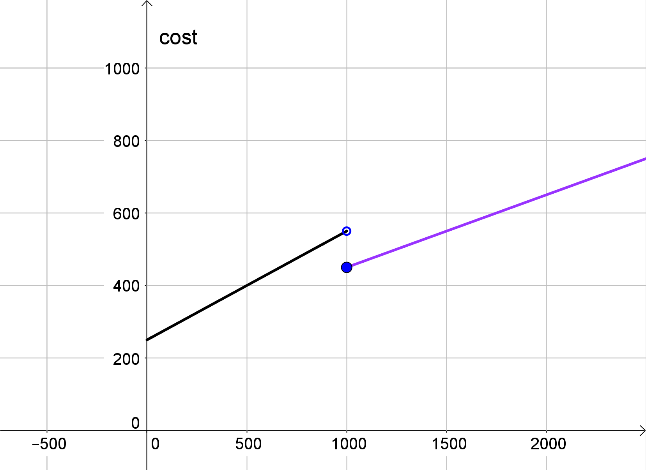
\includegraphics[width=1\linewidth]{./src/images/chapter02/chapter02section01-example01-graph.png}
\caption{Graph of \(A(N)\)\label{figure-1}}
\end{figure}
\hypertarget{p-9}{}%
Printing Company B will only accept orders for \(500\) or more posters.  Printing Company B charges nothing for a template and \(\$0.35\) per poster.%
\par
\hypertarget{p-10}{}%
Use the information given about the two printing companies to answer the following questions.%
\leavevmode%
\begin{enumerate}[label=\alph*)]
\item\hypertarget{li-1}{}Suppose that Chuck can spend at most \(\$300\) on posters. How many posters can he afford to have printed if he uses Company A? What if he can spend at most \(\$600\)?%
\item\hypertarget{li-2}{}If Chuck buys \(800\) posters from Company A, he will pay \(A(800) = 250 + 0.30 \cdot 800 = 490\). Show that he could choose to purchase more than \(1,000\) for the same cost.%
\item\hypertarget{li-3}{}Let \(B(N)\) represent the amount of money, in dollars, that Printing Company B charges to print \(N\) posters.  Use the information you have about \(A(N)\) and \(B(N)\) to explain why Company B will be more economical if Chuck wants to print a relative small number of posters, say \(550\).%
\item\hypertarget{li-4}{}Write an expression for \(B(N)\), and use it to confirm that \(B(550)\) \lt A(550)%
\end{enumerate}
\par\smallskip%
\noindent\textbf{Solution}.\hypertarget{solution-1}{}\quad%
\leavevmode%
\begin{enumerate}[label=\alph*)]
\item\hypertarget{li-5}{}\hypertarget{p-11}{}%
If Chuck can spend at most \(\$300\), the number, \(N\), of posters he can have printed must satisfy \(A(N) \leq 300\). Solving the inequality \(250 + 0.3N \lt 300\) yields \(N \lt 166.67\).  Since \(N\) must be an integer, Chuck can print up to \(166\) posters.%
\begin{figure}
\centering
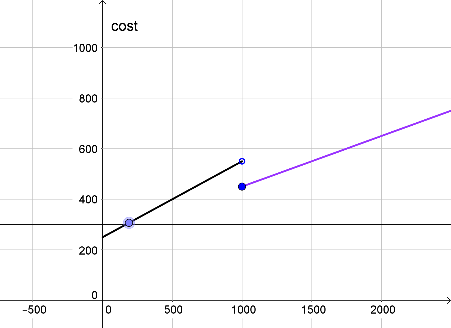
\includegraphics[width=1\linewidth]{./src/images/chapter02/chapter02section01-example01-solutiona-graph.png}
\caption{Graph of \(A(N)\)\label{figure-2}}
\end{figure}
\begin{figure}
\centering
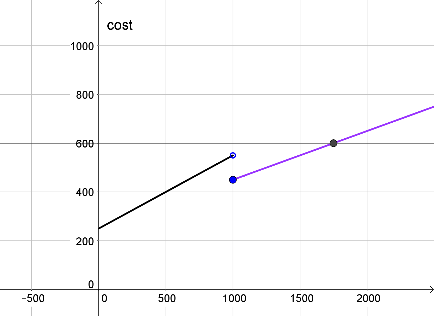
\includegraphics[width=1\linewidth]{./src/images/chapter02/chapter02section01-example01-solutiona-graph2.png}
\caption{Graph of \(A(N)\)\label{figure-3}}
\end{figure}
\hypertarget{p-12}{}%
If Chuck can spend at most \(\$600\), he can print \(N\) posters provided the number \(N\) satisfies \(250 + 0.3N \lt 600\). Solving this inequality shows that yields \(N \lt 1166.67\).  Since \(N\) must be an integer, Chuck can print up to \(1,166\) posters. The graphs on the right illustrate that when \(N \leq 166\), \(A(N) \leq 300\) and when \(N \lt 1166\), \(A(N) \leq 600\)%
\begin{figure}
\centering
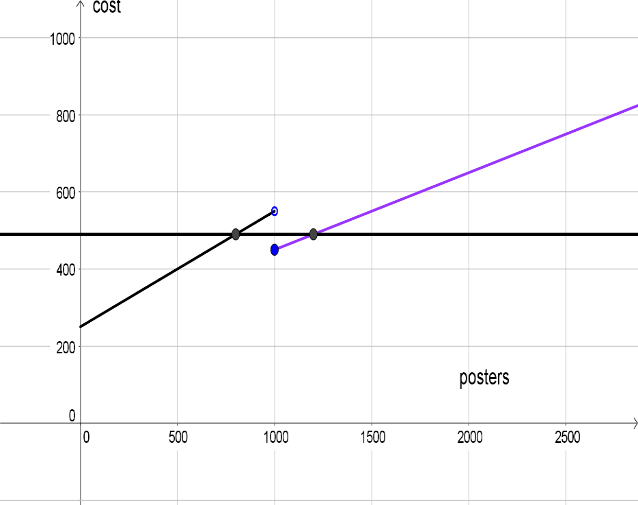
\includegraphics[width=1\linewidth]{./src/images/chapter02/chapter02section01-example01-solutionb-graph.png}
\caption{Graph of \(A(N)\)\label{figure-4}}
\end{figure}
\item\hypertarget{li-6}{}\hypertarget{p-13}{}%
Chuck can spend \(\$490\) to purchase \(800\) posters. He can also purchase \(N\) posters for \(\$490\) if \(N\) satisfies the equation \(250 + 0.20N = 490\). Solving for \(N\) yields \(N = 1,200\). So, Chuck can purchase either \(800\) or \(1,200\) posters for a cost of \(\$490\).%
\item\hypertarget{li-7}{}\hypertarget{p-14}{}%
Company A charges for a template, and since this cost is shared among all the posters printed, the average cost per poster is more than \(\$0.30\). Since company B does not charge for a template and the cost per poster is the only cost, the cost for a small number of posters will less for Company B than for Company A.%
\item\hypertarget{li-8}{}\hypertarget{p-15}{}%
Company B changes \(\$0.35\) for each poster, so \(B(N) = 0.35N\)%
\begin{align*}
A(550) \amp = 250 + 0.30 \cdot 550 = 415\\
B(550) \amp = 0.35 \cdot 550 = 192.5
\end{align*}
As predicted, \(B(550) \lt A(550)\)%
\end{enumerate}
\end{example}
\hypertarget{p-16}{}%
The graph on the left shows \(A(N)\) and \(B(N)\). The graph of \(B(N)\) is continuous because it does not have any breaks. The graph of \(A(N)\) is \emph{discontinuous}; there is a \emph{discontinuity} at \(N = 1,000\).%
\begin{figure}
\centering
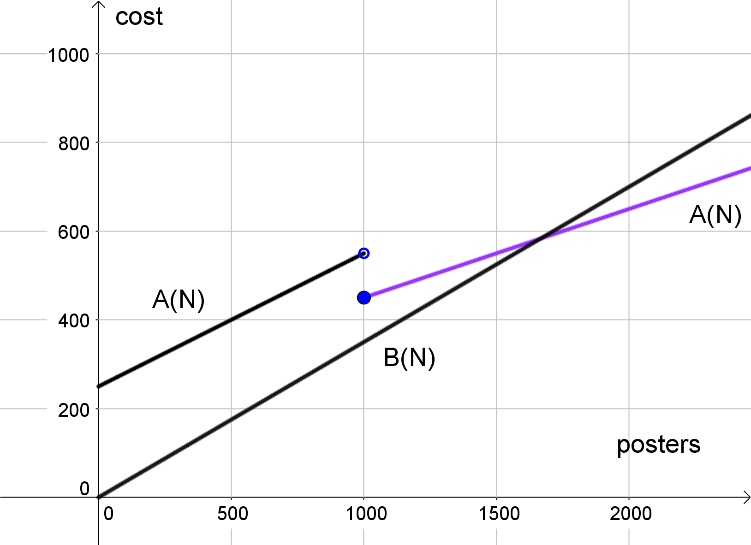
\includegraphics[width=1\linewidth]{./src/images/chapter02/chapter02section01-example01-after-graph.png}
\caption{Graph of \(A(N)\)\label{figure-5}}
\end{figure}
\hypertarget{p-17}{}%
In any situation in which values of one variable are paired with values of another variable, the ordered pairs constitute a \emph{relation}.  All the relationships between variables that we have considered so far are examples of relations.%
\par
\hypertarget{p-18}{}%
Now consider the relation that consists of ordered pairs (distance you fly, price you pay for an airline ticket). You might expect that the cost of an airplane ticket would depend on the distance you fly.  However, it is entirely possible that two tickets for flights of 400 miles might have very different prices.  The price of a ticket is not uniquely determined by the length of the flight. Other factors such as the size of the airports, the day of the week, and the date of the ticket purchase all influence the ticket price.%
\par
\hypertarget{p-19}{}%
The relation between distance and price differs from other relations we have considered.   The difference lies in our ability to use values of the independent variable to predict values of the dependent variable.  Given a value for the independent variable (distance), we cannot confidently determine the value of the dependent variable (price).  In many relations, knowing the value of the independent variable guarantees that we can find a unique value for the dependent variable.  Whenever this is true, the relation is called a function.  In the airplane ticket relation, we are not guaranteed a unique value of the dependent variable; this relation is not a function.%
\par
\hypertarget{p-20}{}%
A \emph{function} is often defined as a set of ordered pairs for which each first coordinate has one and only one second coordinate.  It is also useful to think of a function as a process which maps, or sends, each permissible first coordinate to a unique second coordinate.  Thinking about a function as a mapping emphasizes the process of pairing values.  In this course, it is important to think about functions as being dynamic, as doing something to an x-value to get a y-value.%
\par
\hypertarget{p-21}{}%
A variety of notations are used to define functions.  Functions are usually named with a letter, and \(f\) is a common choice.  The familiar notation \(y = f(x)\), which is read "y equals f of x", shows that \(f\) does something to an \(x\)-value to produce a \(y\)-value.  We could also write \(f: x \rightarrow y\) to show that the function \(f\) sends a value of \(x\) to a particular \(y\). For example, the notations%
\begin{gather*}
f: x \rightarrow x^2 + 1\\
f(x) = x^2 + 1\\
y = x^2 + 1
\end{gather*}
all indicate that a given value of \(x\) is paired with a \(y\)-value that is obtained by squaring the \(x\)-value and then adding \(1\).%
\par
\hypertarget{p-22}{}%
The function \(f\) makes ordered pairs of the form \(\left(x, x^2+1 \right)\). The input is \(x\) and the output is \(x^2 + 1\).  In this notation, \(x\) is often called the argument of the function -- it is the variable that the function acts on to produce the second coordinate of each ordered pair.  The output of the function is sometimes referred to as the value of the function.%
\par
\hypertarget{p-23}{}%
A specialized vocabulary has been developed to help us provide accurate and succinct information about functions. The following examples illustrate some of these mathematical terms and definitions.%
\begin{example}\label{example-2}
\hypertarget{p-24}{}%
After breakfast, a cup of hot chocolate is left sitting on the kitchen table.  When you come home from school, you contemplate drinking the hot chocolate and wonder how its temperature has changed throughout the day.  \hyperref[chapter02-section01-example02-graph]{Figure~8} shows a graph that represents the relationship between the temperature of the hot chocolate and the length of time it has been sitting out.%
\begin{figure}
\centering
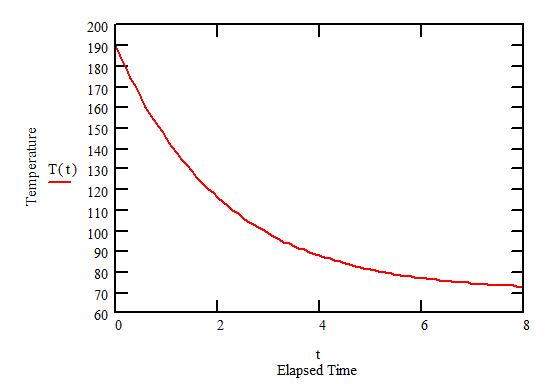
\includegraphics[width=1\linewidth]{./src/images/chapter02/chapter02section01-example02-graph.png}
\caption{Temperature of Hot Chocolate versus Elapsed Time\label{chapter02-section01-example02-graph}}
\end{figure}
\hypertarget{p-25}{}%
Since the temperature depends on the time, the temperature of the hot chocolate is the dependent variable and the amount of time that has passed since the hot chocolate was left on the table is the independent variable.  You can think about a function that has ordered pairs (elapsed time, temperature). The numbers that represent elapsed time make up the \emph{domain} of the function -- they are the first coordinates in the ordered pairs of the function.  In this case you have a limited domain.  Domain values extend from time 0, which represents the time the hot chocolate was put on the table, until you arrived home from school.  If, for example, you were gone eight hours, the domain would be \(0 \leq x \leq 8\).  The numbers that represent the temperatures during this time make up the \emph{range} of the function -- they are the second coordinates in the ordered pairs of the function.%
\par
\hypertarget{p-26}{}%
Judging from the scale on the axes in \hyperref[chapter02-section01-example02-graph]{Figure~8}, we could estimate that the range in this example is \(75 \leq y \leq 190\). This graph doesn’t have an \(x\)-intercept since there is no time at which the temperature is zero.  It does, however, have a \(y\)-intercept.  The \(y\)-intercept represents the temperature when the \(x\)-value equals zero.  In this situation, the y-intercept represents the initial temperature of the drink.  If you examine the graph from left to right beginning at the \(y\)-intercept, you will notice that \(y\)-values continue to decrease as \(x\)-values increase indicating that the temperature continues to fall.   Thus, the function that models the relationship between temperature and time is said to be \emph{decreasing}.  As the values of the independent variable, time, get larger and larger, the values of the dependent variable, temperature, get smaller and smaller.  Another important feature of the graph that shows the temperature decreasing is the upward curvature.  In mathematics, this curvature is called \emph{concave up}.%
\par
\hypertarget{p-27}{}%
In contrast, the graph below shows the temperature of a drink that starts out cold and warms up to room temperature as time passes. The function that models the relationship between temperature and time is \emph{increasing} and its curvature is described as \emph{concave down}.%
\begin{figure}
\centering
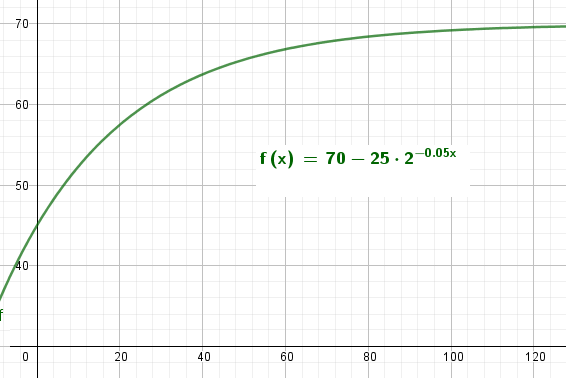
\includegraphics[width=1\linewidth]{./src/images/chapter02/chapter02section01-example02-graph2.png}
\caption{Function that is increasing and concave down\label{chapter02-section01-example02-graph2}}
\end{figure}
\end{example}
\begin{example}\label{example-3}
\leavevmode%
\begin{figure}
\centering
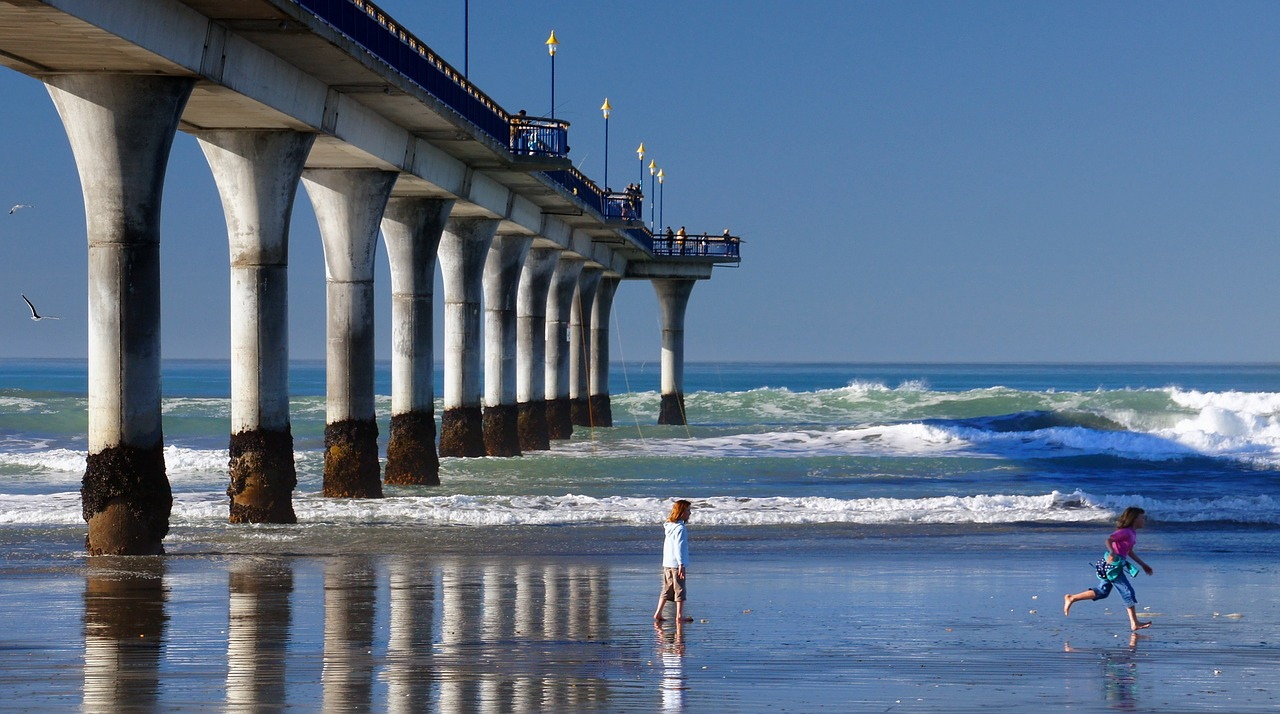
\includegraphics[width=1\linewidth]{./src/images/chapter02/chapter02section01-example03-image.jpg}
\caption{\label{chapter02-section01-example03-image}}
\end{figure}
\hypertarget{p-28}{}%
At low tide, water marks on the supports of a pier reveal the different water levels that have occurred since the preceding low tide. The high-water mark is \(2.2\) meters above the low water mark. The elapsed time between consecutive high-water marks is about \(12.5\) hours.%
\begin{figure}
\centering
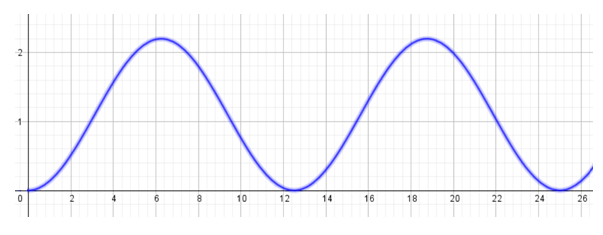
\includegraphics[width=1\linewidth]{./src/images/chapter02/chapter02section01-example03-graph.png}
\caption{Water level on pier posts\label{chapter02-section01-example03-graph}}
\end{figure}
\hypertarget{p-29}{}%
A function that models this situation consists of ordered pairs (elapsed time, water height).  The domain is all real numbers greater than or equal to zero, written \(x \geq 0\).  Since the height of the water is measured relative to the height at low tide, the range is all real numbers in the interval \(0 \leq y \leq 2.2\). The graph contains the point \(\left( 0, 0 \right)\) because the tide was low and the water height was zero when \(x = 0\). Thus the \(x\)-intercepts of the graph represent times associated with low tide. These \(x\)-values that produce a \(y\)-value of zero are called \emph{zeros} of the function. The peaks on the graph occur at times associate with high tide. The peaks occur at times that are separated by \(12.5\) hours. The points associated with both low tide and high tide can be described as turning points.  At a turning point, a function changes from increasing to decreasing or vice versa.  The function graphed in \hyperref[chapter02-section01-example03-graph]{Figure~12} has infinitely many turning points.  This function also changes curvature many times.  At times midway between a low tide and the next high tide, the graph changes from concave up to concave down. At times midway between a high tide and the next low tide, the curvature changes from concave down to concave up.%
\end{example}
\typeout{************************************************}
\typeout{Exercises 1.1 Exercises}
\typeout{************************************************}
\subsection*{Exercises}\hypertarget{exercises-1}{}
\addcontentsline{toc}{subsection}{Exercises}
\begin{divisionexercise}{1}\hypertarget{exercise-1}{}
\hypertarget{p-30}{}%
Refer to \hyperref[chapter02-section01-example01]{Example~1}. Chuck would be unwise to purchase \(N=800\) posters from Company A, because for the same cost, \(\$490\), he could purchase more than \(1,000\) posters form Company A. Find all the other prices for which this situation occurs.%
\end{divisionexercise}%
\begin{divisionexercise}{2}\hypertarget{exercise-2}{}
\hypertarget{p-31}{}%
The examples you have seen in this section include a function that is decreasing and concave up, as well as a function that is increasing and concave down. \leavevmode%
\begin{enumerate}[label=(\alph*)]
\item\hypertarget{li-9}{}Sketch the graph of a function that is decreasing and concave down. Describe a situation that would be represented by your graph.%
\item\hypertarget{li-10}{}Sketch the graph of a function that is increasing and concave up. Describe a situation that would be represented by your graph.%
\end{enumerate}
%
\end{divisionexercise}%
\begin{divisionexercise}{3}\hypertarget{exercise-3}{}
\hypertarget{p-32}{}%
For each relationship described below, identify the two quantities that vary and decide which should be represented by an independent variable and which by a dependent variable. Sketch a reasonable graph to show the relationship between the two variables.  You should only be concerned with the basic shape of the graph, not with particular points.  Write a sentence or two to justify the shape and behavior of your graph. \leavevmode%
\begin{enumerate}[label=\alph*)]
\item\hypertarget{li-11}{}The amount of money earned for a part-time job and the number of hours worked.%
\item\hypertarget{li-12}{}The number of people absent from school each day of the school year.%
\item\hypertarget{li-13}{}The temperature of an ice-cold drink left in a warm room for a period of time.%
\item\hypertarget{li-14}{}The amount of daylight each day of the year.%
\item\hypertarget{li-15}{}The water level on the supports of a pier at an ocean beach on a calm day.%
\item\hypertarget{li-16}{}The population of the U.S. according to each census since 1790.%
\item\hypertarget{li-17}{}The height of a baseball after being hit into the air.%
\item\hypertarget{li-18}{}The distance between the ceiling and the tip of the minute hand of a clock hung on the wall.%
\item\hypertarget{li-19}{}The height of an individual as he or she ages.%
\item\hypertarget{li-20}{}The size of a person's vocabulary from birth onwards.%
\item\hypertarget{li-21}{}The number of bacteria in a culture over a period of time.%
\end{enumerate}
%
\end{divisionexercise}%
\begin{divisionexercise}{4}\hypertarget{exercise-4}{}
\hypertarget{p-33}{}%
Sketch a graph of the relationship presented in each table.  Identify dependent and independent variables.  State any conclusions you can make about the relationship based on the shape of your graph. \leavevmode%
\begin{enumerate}[label=\alph*)]
\item\hypertarget{li-22}{}%
\item\hypertarget{li-23}{}%
\end{enumerate}
%
\begin{figure}
\centering
\begin{tabular}{cc}\hrulemedium
\multicolumn{1}{l}{Weight}&\multicolumn{1}{l}{Rate}\tabularnewline\hrulemedium
\multicolumn{1}{l}{not more than 1 oz}&\(0.32\)\tabularnewline[0pt]
\multicolumn{1}{l}{greater than 1 and not more than 2 ozs}&\(0.55\)\tabularnewline[0pt]
\multicolumn{1}{l}{greater than 2 and not more than 3 ozs}&\(0.78\)\tabularnewline[0pt]
\multicolumn{1}{l}{greater than 3 and not more than 4 ozs}&\(1.01\)\tabularnewline[0pt]
\multicolumn{1}{l}{greater than 4 and not more than 5 ozs}&\(1.24\)\tabularnewline[0pt]
\multicolumn{1}{l}{greater than 5 and not more than 6 ozs}&\(1.47\)\tabularnewline[0pt]
\multicolumn{1}{l}{greater than 6 and not more than 7 ozs}&\(1.70\)\tabularnewline[0pt]
\multicolumn{1}{l}{greater than 7 and not more than 8 ozs}&\(1.93\)\tabularnewline[0pt]
\multicolumn{1}{l}{greater than 8 and not more than 9 ozs}&\(2.16\)\tabularnewline[0pt]
\multicolumn{1}{l}{greater than 9 and not more than 10 ozs}&\(2.39\)\tabularnewline[0pt]
\multicolumn{1}{l}{greater than 10 and not more than 11 ozs}&\(2.62\)\tabularnewline[0pt]
\multicolumn{1}{l}{greater than 11 and not more than 13 ozs}&\(2.90\)\tabularnewline[0pt]
greater than 13 and not more than 16oz&\(2.95\)\tabularnewline\hrulemedium
\end{tabular}
\caption{Third Class Postage Rates\label{chapter02-section01-postage-table}}
\end{figure}
\begin{figure}
\centering
\begin{tabular}{cc}\hrulemedium
\multicolumn{1}{l}{Taxable Income}&\multicolumn{1}{l}{Income Tax}\tabularnewline\hrulemedium
\multicolumn{1}{l}{over \(\$0\) but not over \(\$23,350\)}&\(15 \%\)of income\tabularnewline[0pt]
\multicolumn{1}{l}{over \(\$23,350\) but not over \(\$56,550\)}&\(\$3,502.50 + 28 \%\) of income over \(\$23,350\)\tabularnewline[0pt]
\multicolumn{1}{l}{over \(\$56,550\) but not over \(\$117,950\)}&\(\$12,798.50 + 31 \%\) of income over \(\$56,550\)\tabularnewline[0pt]
\multicolumn{1}{l}{over \(\$117,950\) but not over \(\$256,50\)}&\(\$31,832.50 + 36 \%\) of income over \(\$117,950\)\tabularnewline[0pt]
\multicolumn{1}{l}{over \(\$256,500\)}&\(\$81,710.50 + 39.6\%\) of income over \(\$256,500\)\tabularnewline\hrulemedium
\end{tabular}
\caption{Income Tax Table\label{chapter02-section01-income-table}}
\end{figure}
\end{divisionexercise}%
\begin{divisionexercise}{5}\hypertarget{exercise-5}{}
\hypertarget{p-34}{}%
Let \(f(x) = 3x - 1\). \leavevmode%
\begin{enumerate}[label=(\alph*)]
\item\hypertarget{li-24}{}Find \(f(4)\).%
\item\hypertarget{li-25}{}Find \(x\) such that \(f(x) = 4\).%
\item\hypertarget{li-26}{}Write an expression for \(f(2x), 2f(x), f\left(x+2\right),\) and \(f(x) + 2\)%
\end{enumerate}
%
\end{divisionexercise}%
\begin{divisionexercise}{6}\hypertarget{exercise-6}{}
\hypertarget{p-35}{}%
Let \(g(x) = x^2 - x\). \leavevmode%
\begin{enumerate}[label=(\alph*)]
\item\hypertarget{li-27}{}Write an expression for \(g(a)\).%
\item\hypertarget{li-28}{}Find \(x\) such that \(g(x) = 6\).%
\item\hypertarget{li-29}{}Find \(x\) such that \(g(x) = -6\)%
\item\hypertarget{li-30}{}Write an expression for \(g\left( \frac{1}{x} \right), \frac{1}{g(x)}, g(x-1)\) and \(g(x) - 1\)%
\end{enumerate}
%
\end{divisionexercise}%
\begin{divisionexercise}{7}\hypertarget{exercise-7}{}
\hypertarget{p-36}{}%
Suppose that \(f(x) = 4x - x^2\) and \(g(x) = \sqrt{3x} - 5\). Simplify each given expression. \leavevmode%
\begin{enumerate}[label=(\alph*)]
\item\hypertarget{li-31}{}\(f(-x)\)%
\item\hypertarget{li-32}{}\(g(2x) + 1\)%
\item\hypertarget{li-33}{}\(g\left(x^2\right) + 4\)%
\item\hypertarget{li-34}{}\(3f(x) - g(x) + 2\)%
\item\hypertarget{li-35}{}\(g(x-2)\)%
\item\hypertarget{li-36}{}\(f(x+1)\)%
\item\hypertarget{li-37}{}\(\frac{f(x+h)-f(x)}{h}\)%
\end{enumerate}
%
\end{divisionexercise}%
\begin{divisionexercise}{8}\hypertarget{exercise-8}{}
\hypertarget{p-37}{}%
If \(f(x) = x^2 + x\), write and simplify an expression for each of the following: \leavevmode%
\begin{enumerate}[label=(\alph*)]
\item\hypertarget{li-38}{}\(f(x+1)\)%
\item\hypertarget{li-39}{}\(2f(x)-3\)%
\item\hypertarget{li-40}{}\(f\left(\frac{x}{2}\right)\)%
\item\hypertarget{li-41}{}\(f\left(\frac{1}{x}\right)\)%
\item\hypertarget{li-42}{}\(f\left(\lvert| x \rvert \right)\)%
\item\hypertarget{li-43}{}\(f(x+h)\)%
\end{enumerate}
%
\end{divisionexercise}%
\begin{divisionexercise}{9}\hypertarget{exercise-9}{}
\hypertarget{p-38}{}%
Let \(f(x) = x^2\) and let \(g(x) = \frac{1}{x}\). Express each of the following functions as a transformation of \(f\) or \(g\). For instance, the function \(y = \left( x-1 \right)^2\) can be expressed as \(y = f(x+1)\). \leavevmode%
\begin{enumerate}[label=(\alph*)]
\item\hypertarget{li-44}{}\(y = (x-4)^2\)%
\item\hypertarget{li-45}{}\(y = \frac{3}{x}\)%
\item\hypertarget{li-46}{}\(y = x^2 + 5\)%
\item\hypertarget{li-47}{}\(y = \frac{1}{x-1}\)%
\item\hypertarget{li-48}{}\(y = 2 + 7x^2\)%
\item\hypertarget{li-49}{}\(y = \frac{1}{5x}\)%
\end{enumerate}
%
\end{divisionexercise}%
\begin{divisionexercise}{10}\hypertarget{chapter02-section01-exercise10}{}
\hypertarget{p-39}{}%
The function \(y = f(x)\) is graphed below: \begin{figure}
\centering
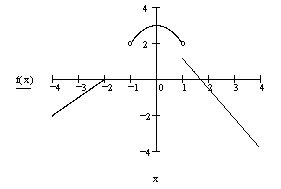
\includegraphics[width=1\linewidth]{./src/images/chapter02/chapter02section01-exercise10-graph.png}
\caption{Graph of \(y = f(x)\)\label{chapter02-section01-exercise10-graph}}
\end{figure}
 \leavevmode%
\begin{enumerate}[label=(\alph*)]
\item\hypertarget{li-50}{}What is the domain of \(f\)?%
\item\hypertarget{li-51}{}What is the range of \(f\)?%
\item\hypertarget{li-52}{}At what \(x\)-value is \(f\) an increasing function? A decreasing function?%
\item\hypertarget{li-53}{}At what \(x\)-values is \(f\) concave up? Concave down?%
\end{enumerate}
%
\end{divisionexercise}%
\typeout{************************************************}
\typeout{Section 1.2 A Toolkit of Functions}
\typeout{************************************************}
\section[{A Toolkit of Functions}]{A Toolkit of Functions}\label{chapter02-section02}
\typeout{************************************************}
\typeout{Subsection 1.2.1 Graphing Functions-Developing a Toolkit}
\typeout{************************************************}
\subsection[{Graphing Functions-Developing a Toolkit}]{Graphing Functions-Developing a Toolkit}\label{subsection-1}
\hypertarget{p-40}{}%
One of the goals of this course is to develop your ability to picture relationships between variables.  This ability includes graphing functions.  To be proficient, you must be able to recognize what functions are best left to a computer or calculator to graph and which are more efficiently tackled with paper and pencil.  In this chapter we will develop knowledge and techniques to facilitate paper-and-pencil graphing.%
\par
\hypertarget{p-41}{}%
Most of the graphs you make by hand do not require pinpoint accuracy.  Rather, your graphs should display basic characteristics of the function and of the relationship between the variables.  To begin, we will discuss a collection of nine functions that make up our \emph{toolkit}. These functions are important for their intrinsic mathematical content and as a set of tools for mathematicians, scientists, economists, and anyone else who creates mathematical models to solve problems.  This toolkit is not sufficient to tackle every problem, but it gives us some common ground that we will use as we expand our knowledge of functions.  A thorough understanding of these toolkit functions is essential and will make the future study of functions and mathematical modeling more meaningful. As you read about each of the nine toolkit functions you should plot a few points to help you understand the graph.%
\typeout{************************************************}
\typeout{Subsection 1.2.2 Constant Function}
\typeout{************************************************}
\subsection[{Constant Function}]{Constant Function}\label{subsection-2}
\hypertarget{p-42}{}%
One of the simplest functions is one in which all first coordinates are paired with the same second coordinate; such a function is called a constant function.  For instance, \(f(x) = 4\) consists of ordered pairs all with second coordinate \(4\).  The graph is the horizontal line \(y = 4\) (see \hyperref[chapter02-section02-constant-and-linear]{Figure~\ref{chapter02-section02-constant-and-linear}} ).%
\begin{figure}
\centering
\begin{sidebyside}{2}{0}{0}{0}
\begin{sbspanel}{0.5}
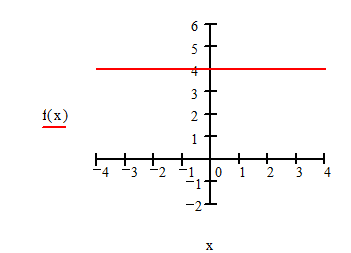
\includegraphics[width=1\linewidth]{./src/images/chapter02/chapter02section02-constant-a.png}
\end{sbspanel}
\begin{sbspanel}{0.5}
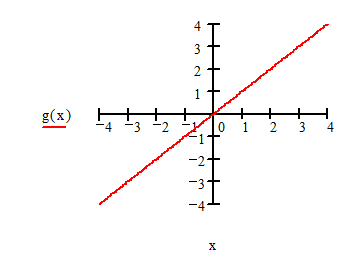
\includegraphics[width=1\linewidth]{./src/images/chapter02/chapter02section02-constant-b.png}
\end{sbspanel}
\end{sidebyside}
\caption{Constant and Linear Functions\label{chapter02-section02-constant-and-linear}}
\end{figure}
\typeout{************************************************}
\typeout{Subsection 1.2.3 Linear Function}
\typeout{************************************************}
\subsection[{Linear Function}]{Linear Function}\label{subsection-3}
\hypertarget{p-43}{}%
The simplest linear function is \(f(x) = x\).  It is often called the identity function because the first and second coordinates in each ordered pair are identical.  The graph of this function is the diagonal line shown in \hyperref[chapter02-section02-constant-and-linear]{Figure~\ref{chapter02-section02-constant-and-linear}}.  Notice that this graph is everywhere increasing and continuous.  The general linear function is \(f(x) = mx+ b\); its graph is a variation of the line \(y = x\) that has slope \(m\) and \(y\)-intercept \(b\).  You should be familiar with these variations from study in previous mathematics courses and from your work in Chapter 1.%
\typeout{************************************************}
\typeout{Subsection 1.2.4 Quadratic Function}
\typeout{************************************************}
\subsection[{Quadratic Function}]{Quadratic Function}\label{subsection-4}
\hypertarget{p-44}{}%
The toolkit \emph{quadratic function} is \(f(x) = x^2\).  You can understand the shape of the graph of \(f(x) = x^2\) by thinking about the ordered pairs \(\left( x , x^2 \right)\) that belong to the function.  Whenever \(x\) is greater than \(1\), \(x^2 \gt x\) so the graph is above the line \(y = x\).  When \(x\) is between \(0\) and \(1\), \(x^2 \lt x\) and the graph is below that of \(y = x\).  The graph of \(f(x) = x^2\), shown in \hyperref[chapter02-section02-quadratic]{Figure~\ref{chapter02-section02-quadratic}} , is called a \emph{parabola}.  Notice that it is decreasing for negative \(x\)-values and increasing for positive \(x\)-values.  The graph has a turning point at \(\left( 0, 0 \right)\), which is called the \emph{vertex} of the parabola.  The curvature of this graph is concave up.%
\begin{figure}
\centering
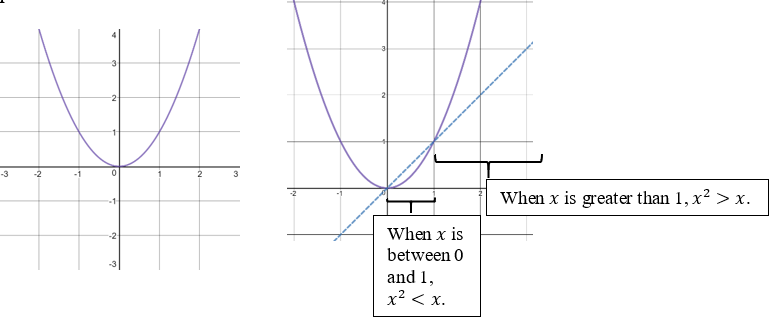
\includegraphics[width=1\linewidth]{./src/images/chapter02/chapter02section02-quadratic.png}
\caption{Quadratic Functions\label{chapter02-section02-quadratic}}
\end{figure}
\typeout{************************************************}
\typeout{Subsection 1.2.5 Cubic Function}
\typeout{************************************************}
\subsection[{Cubic Function}]{Cubic Function}\label{subsection-5}
\hypertarget{p-45}{}%
The graph of the toolkit \emph{cubic} function  \(f(x) =x^3\) is shown in \hyperref[chapter02-section02-cubic]{Figure~\ref{chapter02-section02-cubic}}.  This graph is increasing for all \(x\)-values, and it is steeper than the graph of \(f(x) = x^2\) for \(x \gt 1\). Notice that the graph lies entirely in the first and third quadrants; in the ordered pairs \(\left( x, x^3 \right)\), either both coordinates are positive or both are negative.%
\begin{figure}
\centering
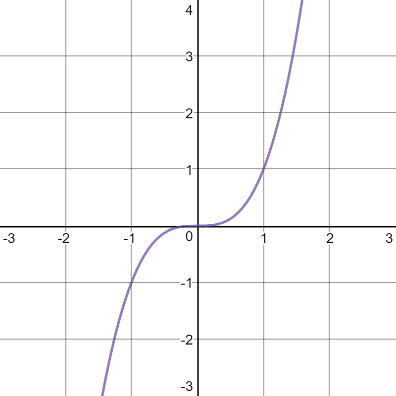
\includegraphics[width=0.5\linewidth]{./src/images/chapter02/chapter02section02-cubic.png}
\caption{Cubic Function\label{chapter02-section02-cubic}}
\end{figure}
\typeout{************************************************}
\typeout{Subsection 1.2.6 Square Root Function}
\typeout{************************************************}
\subsection[{Square Root Function}]{Square Root Function}\label{subsection-6}
\hypertarget{p-46}{}%
The \emph{square root function} is defined by the equation \(f(x) = \sqrt{x}\).  Since the symbol \(\sqrt{x}\) represents only the \emph{principal} (positive) \emph{square root} of \(x\), each \(x\)-value is paired with a unique \(y\)-value.  (Think about what your calculator does when you compute the square root of \(9\); the calculator gives a display of \(3\), not \(\pm 3\)).  The graph of \(f(x) = \sqrt{x}\) is shown in \hyperref[chapter02-section02-root-exp]{Figure~\ref{chapter02-section02-root-exp}}.  Notice that it is increasing for all \(x\)-values, but the rate of increase is very slow.  The curvature of this graph is concave down.%
\par
\hypertarget{p-47}{}%
We can compare the steepness of \(f(x) = \sqrt{x}\) with that of linear, quadratic, and cubic functions by determining for each function the \(x\)-value that is paired with a \(y\)-value of \(64\). For \(f(x) = x^3\), the ordered pair is \(\left( 4, 64 \right)\).    For \(f(x) = x^2\), the ordered pair is \(\left( 8, 64 \right)\). For \(f(x) = x\), the ordered pair is \(\left( 64, 64 \right)\).  For \(f(x) = \sqrt{x}\), the ordered pair is \(\left( 4096, 64 \right)\). Notice that the cubic function attains the value of \(64\) when \(x = 4\), whereas the square root function doesn't attain this value until \(x = 4096\).%
\par
\hypertarget{p-48}{}%
It is also interesting to study the steepness of \(f(x) = \sqrt{x}\) in another way.  When \(x \gt 1\), \(\sqrt{x} \lt x\), so the graph is below the line \(y = x\). In effect, taking the square root pulls \(y\)-values down if \(x \gt 1\). On the other hand, when \(0 \lt x \lt 1\), \(sqrt{x} \gt x\) and the graph is above the line \(y = x\).  For these \(x\)-values, taking the square root increases the \(y\)-values.%
\begin{figure}
\centering
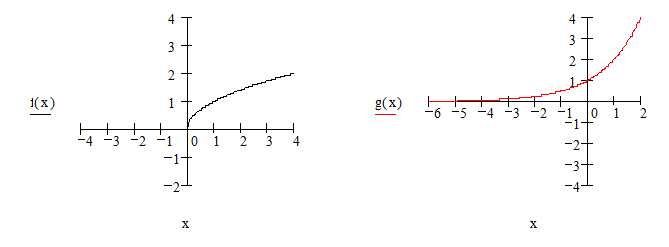
\includegraphics[width=1\linewidth]{./src/images/chapter02/chapter02section02-root-exp.png}
\caption{Square Root and Exponential Functions\label{chapter02-section02-root-exp}}
\end{figure}
\typeout{************************************************}
\typeout{Subsection 1.2.7 Exponential Function}
\typeout{************************************************}
\subsection[{Exponential Function}]{Exponential Function}\label{subsection-7}
\hypertarget{p-49}{}%
The toolkit \emph{exponential function} is \(f(x) = 2^x\).  The graph, shown in \hyperref[chapter02-section02-root-exp]{Figure~\ref{chapter02-section02-root-exp}}, is increasing and concave up for all \(x\)-values.  As the \(x\)-values get more and more negative, \(y\)-values get smaller and approach zero, so the graph gets closer and closer to the negative \(x\)-axis.  We say that the graph is asymptotic to the \(x\)-axis.  In general, any function of the form \(f(x) = a \cdot b^x\), where \(a\) is any nonzero constant, \(b \gt 0\), and \(b \neq 1\), is called an \emph{exponential function}.%
\typeout{************************************************}
\typeout{Subsection 1.2.8 Reciprocal Function}
\typeout{************************************************}
\subsection[{Reciprocal Function}]{Reciprocal Function}\label{subsection-8}
\hypertarget{p-50}{}%
The graph of the \emph{reciprocal function} \(f(x) = \frac{1}{x}\) is shown in \hyperref[chapter02-section02-root-exp]{Figure~\ref{chapter02-section02-root-exp}}.  Notice that the graph is discontinuous at \(x = 0\). The function \(f\) produces an output by taking the reciprocal of its input.  Since taking the reciprocal does not cause a sign change, the graph lies entirely in the first and third quadrants.  In the first quadrant where \(x\)-values are positive, the reciprocals of small numbers are big numbers and the reciprocals of big numbers are small numbers. As \(x\)-values get larger, \(y\)-values get smaller and approach zero, so the graph gets closer and closer to the \(x\)-axis which is an asymptote for the function.  Because, \(x\)-values close to zero are paired with large \(y\)-values, the graph also has the \(y\)-axis as an asymptote.  Similar analysis for negative values of \(x\) explains the behavior of the graph in the third quadrant.%
\begin{figure}
\centering
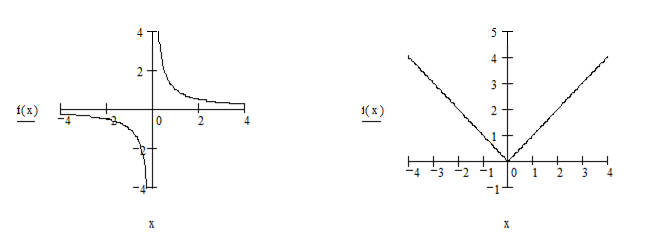
\includegraphics[width=1\linewidth]{./src/images/chapter02/chapter02section02-reciprocal.png}
\caption{Reciprocal and Absolute Value Functions\label{chapter02-section02-recip-abs}}
\end{figure}
\typeout{************************************************}
\typeout{Subsection 1.2.9 Absolute Value Function}
\typeout{************************************************}
\subsection[{Absolute Value Function}]{Absolute Value Function}\label{subsection-9}
\hypertarget{p-51}{}%
The graph on the right in \hyperref[chapter02-section02-root-exp]{Figure~\ref{chapter02-section02-root-exp}} resembling the shape of the letter "V" is the toolkit absolute value function, \(f(x) = \lvert x \rvert\).  Recall that the symbol \(\lvert x \rvert\) is defined as follows:%
%
\begin{gather*}
\lvert x \rvert = x \text{ if } x \geq 0\\
\text{and}\\
\lvert x \rvert = -x \text{ if } x \lt 0
\end{gather*}
\hypertarget{p-52}{}%
For positive \(x\)-values and zero, \(\lvert x \rvert\) is equal to \(x\). For negative \(x\)-values, \(\lvert x \rvert\) is equal to the opposite of \(x\).  The absolute value function is actually an example of a piecewise-defined function.  This means that the function is defined differently for different \(x\)-values.  The function \(f(x) = \lvert x \rvert\) is the same as the piecewise-defined function:%
%
\begin{align*}
f(x) =
\begin{cases}
x, \amp  \ \text{if}  \ x \geq 0 \\
-x, \amp  \ \text{if}  \ x \lt 0 \\
\end{cases}
\end{align*}
\hypertarget{p-53}{}%
Notice that \(f\) pairs positive \(x\)-values with themselves and pairs negative \(x\)-values with their opposites. For positive \(x\)-values the graph of \(f\) is identical to the line \(y = x\); for negative \(x\)-values the graph is identical to the line \(y = -x\).%
\begin{example}\label{example-4}
\hypertarget{p-54}{}%
Sketch a graph of the following piecewise-defined function.%
%
\begin{align*}
f(x) =
\begin{cases}
x^2, \amp  \ \text{if}  \ x \leq -1 \\
\frac{1}{x}, \amp  \ \text{if}  \ -1 \lt x \lt 0 \\
2^x, \amp  \ \text{if}  \ x \geq 0 \\
\end{cases}
\end{align*}
\par\smallskip%
\noindent\textbf{Solution}.\hypertarget{solution-2}{}\quad%
\hypertarget{p-55}{}%
The graph is shown in \hyperref[chapter02-section02-piecewise-soln]{Figure~\ref{chapter02-section02-piecewise-soln}}.  For \(x\)-values less than or equal to \(-1\), the function is defined by the equation \(y = x^2\), and the graph consists of a section of the toolkit parabola.  For \(x\)-values between \(-1\) and \(0\), the function is defined by the equation \(y = \frac{1}{x}\), and the graph consists of a section of the toolkit reciprocal function.  Note the open circle at \(\left( -1, -1 \right)\); this indicates that the point is not on the graph of the function. For \(x\)-values greater than or equal to \(0\), the function is defined by the equation \(y = 2^x\).%
\begin{figure}
\centering
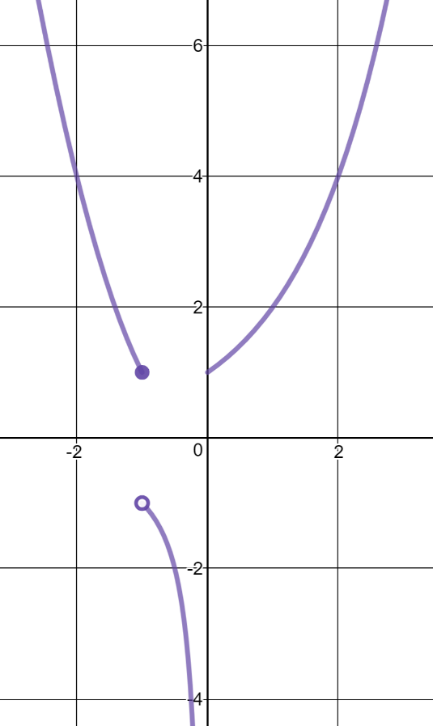
\includegraphics[width=0.5\linewidth]{./src/images/chapter02/chapter02-section02-piecewise-soln.png}
\caption{Graph of Piecewise-Defined Function\label{chapter02-section02-piecewise-soln}}
\end{figure}
\end{example}
\typeout{************************************************}
\typeout{Subsection 1.2.10 Other Useful Functions}
\typeout{************************************************}
\subsection[{Other Useful Functions}]{Other Useful Functions}\label{subsection-10}
\hypertarget{p-56}{}%
There are a few more types of functions that, while not generally thought of as \emph{toolkit functions}, are useful functions to know and understand.%
\typeout{************************************************}
\typeout{Subsection 1.2.11 Power Functions}
\typeout{************************************************}
\subsection[{Power Functions}]{Power Functions}\label{subsection-11}
\hypertarget{p-57}{}%
Functions of the form \(f(x) = a \cdot x^n\) where \(a \neq 0\) and \(n\) is a real number are called \emph{power functions}. The behavior of power functions varies widely depending on the value of \(n\).  If \(n \lt 0\), then \(f(x) = a \cdot x^n\) can be thought of as \(f(x) = \frac{a}{x^{\lvert n \rvert}}\).  In this case, \(f\) has a vertical asymptote at \(x = 0\) and a horizontal asymptote at \(y = 0\). An example of this is shown at the left in \hyperref[chapter02-section02-power]{Figure~\ref{chapter02-section02-power}}.  If \(n \gt 0\), then \(f(x) = a \cdot x^n\) has no asymptotes, and \(\lvert y \rvert\) increases without bound as \(\lvert x \rvert\) increases (see the second and third graphs in \hyperref[chapter02-section02-power]{Figure~\ref{chapter02-section02-power}}).  Notice also that when \(n \gt 0\), all power functions contain the point \(\left( 0, 0 \right)\), and \(f(x) = a \cdot x^n\) contains the point \(\left( 1, a \right)\) for all values of \(n\).%
\begin{figure}
\centering
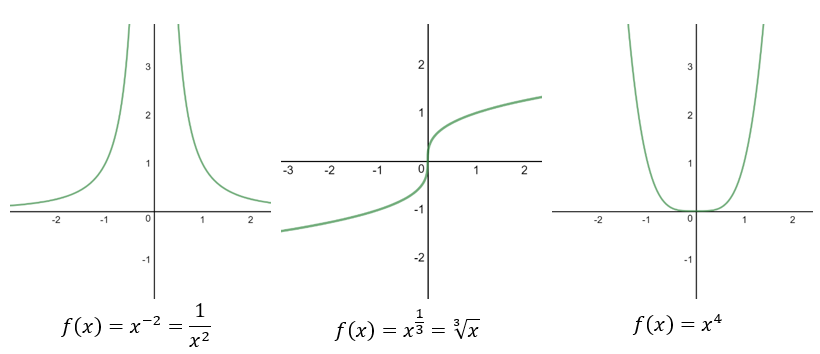
\includegraphics[width=1\linewidth]{./src/images/chapter02/chapter02section02-power.png}
\caption{Graphs of power functions\label{chapter02-section02-power}}
\end{figure}
\typeout{************************************************}
\typeout{Subsection 1.2.12 Triangle Wave Function}
\typeout{************************************************}
\subsection[{Triangle Wave Function}]{Triangle Wave Function}\label{subsection-12}
\hypertarget{p-58}{}%
The triangle wave function defined by the equation \(f(x) = tri(x)\) is graphed in \hyperref[chapter02-section02-twave]{Figure~\ref{chapter02-section02-twave}}. The graph of the triangle wave function oscillates in a regular pattern between a maximum  \(y\)-value of \(1\) and a minimum \(y\)-value of \(-1\).%
\begin{figure}
\centering
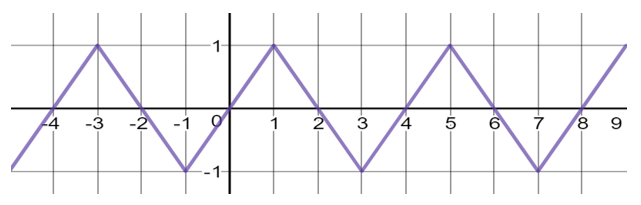
\includegraphics[width=1\linewidth]{./src/images/chapter02/chapter02section02-twave.png}
\caption{Graphs of power functions\label{chapter02-section02-twave}}
\end{figure}
\hypertarget{p-59}{}%
The function has a value of \(0\) at \(x = 0\).  It increases to its maximum of \(1\) at \(x = 1\), returns to \(0\) at \(x = 2\), decreases to its minimum of \(-1\) at \(x = 3\), and returns to \(0\) at \(x = 4\).  Then it repeats the process indefinitely.  If you look at the section of the triangle wave function between \(-4\) and \(0\), or between \(4\) and \(8\), you notice that it has the same shape as the section between \(0\) and \(4\).  Thus the triangle wave function is periodic.  Since the portion being repeated is \(4\) units long, the period is said to be \(4\).  That is, the triangle wave function completes one cycle every \(4\) units.  For those of you who have studied trigonometry, the triangle wave function may remind you of the sine function.  This is a similar periodic function that we will study and add to our toolkit of functions later in the course.%
\typeout{************************************************}
\typeout{Subsection 1.2.13 Greatest Integer Function}
\typeout{************************************************}
\subsection[{Greatest Integer Function}]{Greatest Integer Function}\label{subsection-13}
\hypertarget{p-60}{}%
The symbol \(\left\lfloor x \right\rfloor\) denotes the greatest integer that is less than or equal to \(x\).  For example,  \(\left\lfloor 11.02 \right\rfloor = 11, \left\lfloor 4.9 \right\rfloor = 4, \left\lfloor 2 \right\rfloor = 2\),  and \(\left\lfloor -2.4 \right\rfloor = -3\).  The function \(f(x) = \left\lfloor x \right\rfloor\) is called the \emph{greatest integer} or \emph{floor function}. For any \(x\)-value between \(0\) and \(1\), \(f(x) = 0\), so over this part of the domain \(f\) behaves like a constant function. Similarly, for any \(x\)-value between \(1\) and \(2\),  \(f(x) = 1\). Thus, the graph of \(f\) consists of a collection of horizontal line segments, or \emph{steps}. The graph is shown in \hyperref[chapter02-section02-floor]{Figure~\ref{chapter02-section02-floor}}.  Note that it is discontinuous at every integer value of \(x\).  Identify the domain and the range of the function \(f(x) = \left\lfloor x \right\rfloor\).%
\begin{figure}
\centering
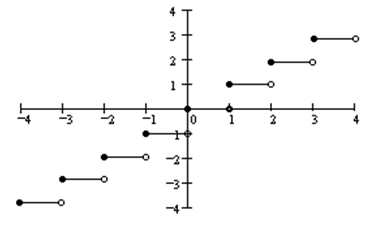
\includegraphics[width=1\linewidth]{./src/images/chapter02/chapter02section02-floor.png}
\caption{Graphs of Greatest Integer function\label{chapter02-section02-floor}}
\end{figure}
\typeout{************************************************}
\typeout{Exercises 1.2 Exercises}
\typeout{************************************************}
\subsection*{Exercises}\hypertarget{exercises-2}{}
\addcontentsline{toc}{subsection}{Exercises}
\begin{divisionexercise}{1}\hypertarget{exercise-11}{}
\hypertarget{p-61}{}%
Sketch graphs of \(y = x^4, y=x^5, y=x^6\) and \(y=x^7\). Make a generalization about the graph of \(y=x^n\) for \(n\) an even positive integer and for \(n\) an odd positive integer.%
\end{divisionexercise}%
\begin{divisionexercise}{2}\hypertarget{exercise-12}{}
\hypertarget{p-62}{}%
Identify the domain and the range of each toolkit function.%
\end{divisionexercise}%
\begin{divisionexercise}{3}\hypertarget{exercise-13}{}
\hypertarget{p-63}{}%
Which toolkit functions are examples of power functions?%
\end{divisionexercise}%
\begin{divisionexercise}{4}\hypertarget{exercise-14}{}
\hypertarget{p-64}{}%
Let \(p(x) = \sqrt{x}, q(x) = \frac{1}{x}\),and \(r(x) = x^3\). Express each of the following as a transformation of \(p, q\), or \(r\). For instance, \(y = \sqrt{ \left( x+1 \right) + 2 }\) can be expressed as \(y = p\left( x + 1 \right) + 2\). \leavevmode%
\begin{enumerate}[label=(\alph*)]
\item\hypertarget{li-54}{}\(y = 1 + \frac{1}{x}\)%
\item\hypertarget{li-55}{}\(y = 8x^3\)%
\item\hypertarget{li-56}{}\(y = \frac{1}{2x - 2}\)%
\item\hypertarget{li-57}{}\(y = \sqrt{6 - x}\)%
\item\hypertarget{li-58}{}\(y = 3 - \sqrt{x}\)%
\item\hypertarget{li-59}{}\(y = \left( 2x \right)^3\)%
\end{enumerate}
%
\end{divisionexercise}%
\begin{divisionexercise}{5}\hypertarget{exercise-15}{}
\hypertarget{p-65}{}%
Use technology to graph \(y=x, y=x^2\), and \(y=x^3\). Set a viewing window of \(0 \leq x \leq 1\) and \(0 \leq y \leq 1\).  Write one or two sentences to compare the three graphs.  How would the graph of \(y=x^4\) look compared to the graphs of these other functions in this window?%
\end{divisionexercise}%
\begin{divisionexercise}{6}\hypertarget{exercise-16}{}
\hypertarget{p-66}{}%
Use a calculator to graph \(y=x\),and \(y=\sqrt{x}\). Set a viewing window of \(0 \leq x \leq 1\) and \(0 \leq y \leq \)1.  Write one or two sentences to compare the graphs.%
\end{divisionexercise}%
\begin{divisionexercise}{7}\hypertarget{exercise-17}{}
\hypertarget{p-67}{}%
The graphs of several toolkit functions exhibit symmetry. The ability to identify symmetries will help you as you learn to graph other functions that do not belong to the toolkit. \leavevmode%
\begin{enumerate}[label=(\alph*)]
\item\hypertarget{li-60}{}\hypertarget{p-68}{}%
Notice when looking at the function \(f(x) = x^2\), the expression for \(f(-x)\) is identical to that for \(f(x)\).%
\begin{gather*}
f(-x) = \left( -x \right)^2 = x^2 = f(x)
\end{gather*}
Since \(f(-x) = f(x)\), for every point \(\left( x, y \right)\) on the graph of \(f\) there is also a point \(\left(-x, y \right)\). The fact that these points have the same \(y\)-coordinate paired with opposite \(x\)-coordinates means that the graph is \emph{symmetric about the \(y\)-axis}. A function that has this type of symmetry is called an \emph{even function}.  Which other toolkit functions are even functions?%
\item\hypertarget{li-61}{}\hypertarget{p-69}{}%
Now look at the toolkit function \(m(x) = x^3\). Note that \(m(-x)\) is not equal to \(m(x)\). But notice that \(m(-x)\) is equal to the opposite of \(m(x)\).%
\begin{gather*}
m(-x) = \left( -x \right)^3 = -x^3 = -m(x)
\end{gather*}
Since \(m(-x) = -m(x)\), for every point \(\left( x, y \right)\) on the graph of \(m\), the point \(\left( -x, -y \right)\) is also on the graph. The graph of \(m\) is \emph{symmetric about the point} \(\left( 0, 0 \right)\). A function with this type of symmetry is called an \emph{odd function}.  Which other toolkit functions are odd functions?%
\end{enumerate}
%
\end{divisionexercise}%
\begin{divisionexercise}{8}\hypertarget{exercise-18}{}
\hypertarget{p-70}{}%
Why are the terms "even" and "odd" reasonable choices to describe functions whose graphs display certain symmetries? \emph{Hint: Think about power functions.}%
\end{divisionexercise}%
\begin{divisionexercise}{9}\hypertarget{exercise-19}{}
\hypertarget{p-71}{}%
Can the graph of a function be both even and odd?  Explain.%
\end{divisionexercise}%
\begin{divisionexercise}{10}\hypertarget{exercise-20}{}
\hypertarget{p-72}{}%
Must a function be either even or odd?  Are there toolkit functions that are neither?  Do they exhibit other types of symmetry?  Explain your answers and give examples to support your conclusions.%
\end{divisionexercise}%
\begin{divisionexercise}{11}\hypertarget{exercise-21}{}
\hypertarget{p-73}{}%
Discuss the symmetry of the graph of \(f(x) = 1 + \frac{1}{x-1}\)%
\begin{figure}
\centering
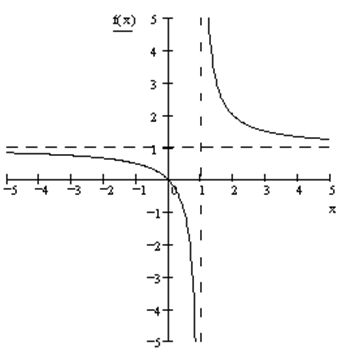
\includegraphics[width=0.5\linewidth]{./src/images/chapter02/chapter02section02-exercise11.png}
\caption{Graph of \(f(x) = 1 + \frac{1}{x-1}\)\label{chapter02-section02-exercise11-figure}}
\end{figure}
\end{divisionexercise}%
\begin{divisionexercise}{12}\hypertarget{exercise-22}{}
\hypertarget{p-74}{}%
\hyperref[chapter02-section02-exercise12-figure]{Figure~\ref{chapter02-section02-exercise12-figure}} shows the graph of a function \(y = h(x)\) for \(0 \leq x \leq 3\). \leavevmode%
\begin{enumerate}[label=(\alph*)]
\item\hypertarget{li-62}{}Sketch the graph of \(h\) from \(-3\) to \(3\) if \(h\) is an even function.%
\item\hypertarget{li-63}{}Sketch the graph of \(h\) from \(-3\) to \(3\) if \(h\) is an odd function.%
\end{enumerate}
%
\begin{figure}
\centering
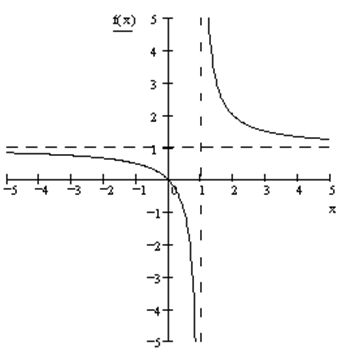
\includegraphics[width=0.5\linewidth]{./src/images/chapter02/chapter02section02-exercise11.png}
\caption{Graph of \(f(x) = 1 + \frac{1}{x-1}\)\label{chapter02-section02-exercise12-figure}}
\end{figure}
\end{divisionexercise}%
\begin{divisionexercise}{13}\hypertarget{exercise-23}{}
\hypertarget{p-75}{}%
Use technology to graph the functions \(f(x) = x^2\) and \(g(x) = 2^x\). Write several sentences comparing the growth of the functions for \(x \gt 0\). How many times do these graphs intersect?  Find the coordinates of all points of intersection%
\end{divisionexercise}%
\begin{divisionexercise}{14}\hypertarget{exercise-24}{}
\hypertarget{p-76}{}%
In defining the exponential function \(f(x) = a \cdot b^x\), we stated that the base \(b\) must be greater than zero. \leavevmode%
\begin{enumerate}[label=(\alph*)]
\item\hypertarget{li-64}{}What problems are associated with negative values of \(b\)?  To help answer this question, consider \(m(x) = \left( -2 \right)^x\) and make a table of values for \(x = -3, -2, -1, -0.5, 0, 0.5, 1, 1.5, 2\), and \(3\). What happens if you try to sketch a graph of \(y = m(x)\)?%
\item\hypertarget{li-65}{}Consider the function \(n(x) = 0^x\). Why does n(0) present a dilemma?%
\end{enumerate}
%
\end{divisionexercise}%
\begin{divisionexercise}{15}\hypertarget{exercise-25}{}
\hypertarget{p-77}{}%
Sketch a graph of each piecewise-defined function. \leavevmode%
\begin{enumerate}[label=(\alph*)]
\item\hypertarget{li-66}{}\(f(x) =
\begin{cases}
x, \amp  \ \text{if}  \ x \geq -2 \\
\lvert x \rvert, \amp  \ \text{if}  \ x \lt -2 \\
\end{cases}\)%
\item\hypertarget{li-67}{}\(f(x) =
\begin{cases}
x^3, \amp  \ \text{if}  \ x \lt 0 \\
2^x, \amp  \ \text{if}  \ x \geq 0 \\
\end{cases}\)%
\item\hypertarget{li-68}{}\(f(x) =
\begin{cases}
x + 2, \amp  \ \text{if}  \ x \leq 0 \\
2, \amp  \ \text{if}  \ 0 \lt x \lt 4 \\
\sqrt{x}, \amp  \ \text{if}  \ x \gt 4 \\
\end{cases}\)%
\item\hypertarget{li-69}{}\(f(x) =
\begin{cases}
1, \amp  \ \text{if}  \ \lvert x \rvert \lt 1 \\
x^2, \amp  \ \text{if}  \ \lvert x \rvert \geq 1 \\
\end{cases}\)%
\end{enumerate}
%
\end{divisionexercise}%
\begin{divisionexercise}{16}\hypertarget{exercise-26}{}
\hypertarget{p-78}{}%
Suppose \(f(x)\) is a linear function and you know that \(f(0) = 4\) and that \({f(x) - f(x-2) = -3}\) for all values of \(x\).  Write an expression for \(f(x)\).%
\end{divisionexercise}%
\end{document}